% !Mode:: "TeX:UTF-8"

\chapter{绪论}


\section{研究背景与意义}

随着移动互联网的广泛部署,智能终端结合各项计算机技术的迅猛发展,基于位置的服务也顺应了时代的发展,位置服务已经成为了人们生活中必不可少的一部分,因此研究人员相继提出了基于无线保真技术 (Wireless-Fidelity,Wi-Fi)、蓝牙、超宽带技术(Ultra-Wideband,UWB)、射频识别技术(Radio Frequency Identification,RFID)等不同的方法尝试在室内环境下提供定位服务。

\textcolor[rgb]{1.00,0.00,0.00}{【正文中所有的数字和字母都用“Times New Roman”字体。】}

\textcolor[rgb]{1.00,0.00,0.00}{【论述清楚为什么选择这个题目来研究,即阐述该研究对学科发展的贡献、对国计民生的理论与现实意义等。】}


位置,与人类社会的生产生活息息相关。自 2010 年以来,伴随传统网络向物理世界延伸的大趋势,位置信息成为物联网最基础的感知信息,是沟通物理世界和数字世界的桥梁。近年来,移动互联网的异军突起,也令位置信息的关键作用愈发凸显。

\section{国内外研究现状分析}

\textcolor[rgb]{1.00,0.00,0.00}{【对本研究主题范围内的文献进行详尽的综合述评,“述”的同时一定要有“评”,指出现有研究状态,仍存在哪些尚待解决的问题,讲出自己的研究有哪些探索性内容。】}

毫无疑问,未来全球性的室内定位服务一定会出现。但今天,室内定位在技术上最终花落谁家,在商业上又将鹿死谁手,都还不得而知。人们憧憬着物联网世界以及即将开启的工业 4.0 时代中“一切皆可感知、一切皆可定位”的美好景象,同时也面临着目前各家定位技术各据一方占“楼”为王的尴尬现实。表 1-1 列举分析了一些室内定位技术的特点,根据表 1-1 的内,多个角度介绍不同技术,对比得出各自的特点。


\section{图、表、公式、算法等的说明}

下面是关于图、表、公式和算法的详细说明。

\subsection{图的说明}

图要求清晰,最好为矢量图(PDF 和 EPS 格式),图中文字最好用中文。

如图\ref{Fig1-1}所示,WSN 是一个包含了传感节点和路由节点两类型节点的网络,这些传感器节点是自治的,并且规模较小。在典型的传感器网络部署结构中,BS 负责从传感器节点收集数据后进行处理。这些部署的传感器节点根据单个事件向路由节点转发数据,将这些信息转发至路由节点或下一个中继节点,并进行处理和聚合。它可以被放置在一个特定的环境中,用来监测诸如风速,温度,土壤 pH 值,二氧化碳浓度等的变化。这些网络收集和处理来自传感器节点的数据,然后通过因特网将其传输至用户。

\begin{figure}[htbp]
\vspace*{6pt}
\centering
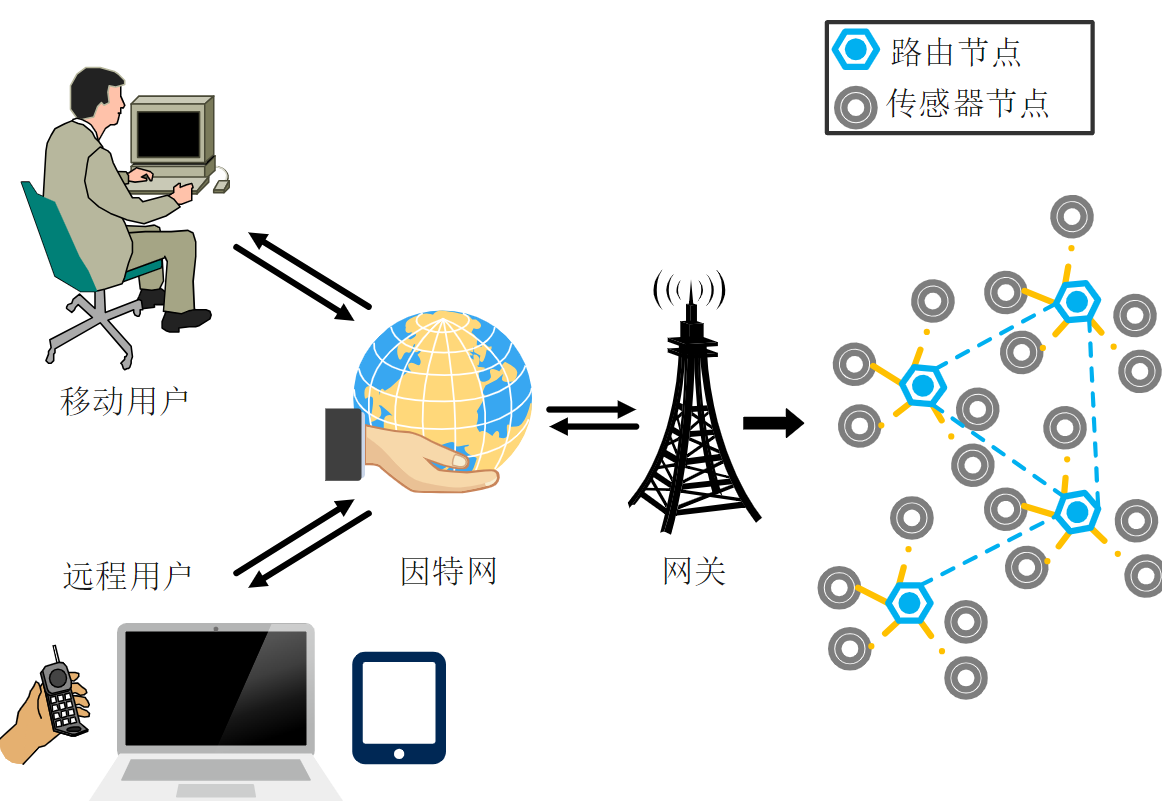
\includegraphics[width=0.75\textwidth]{1-1}
\caption{无线传感器网络体系结构}\label{Fig1-1}
\vspace*{10pt}
\end{figure}


\textcolor[rgb]{1.00,0.00,0.00}{1. 图要精选,具有自明性,切忌与表及文字表述重复。图要清楚,但坐标比例不要过分放大,同一图上不同曲线的点要分别用不同形状的标识符标出。地图插图涉及中国地图全图时,须使用自然资源部标准地图底图制作。}

\textcolor[rgb]{1.00,0.00,0.00}{2. 图序与图名置于图的下方,用宋体 5 号字,居中,段前空 6 磅,段后空 12 磅,单倍行距;图序与图名文字之间空一个字符。如“图 2-1 发展中国家经济增长速度的比较(1960-2000)”,其中“图 2-1”是图序。}

\textcolor[rgb]{1.00,0.00,0.00}{3. 图中的术语、符号、单位等应与正文表述中所用一致,图中文字用 5 号或小 5 号(9~10.5 磅)字,以能够清晰阅读为标准。专用名字代号、单位可采用外文表示,坐标轴题名、词组、描述性的词语均须采用中文。}

\textcolor[rgb]{1.00,0.00,0.00}{4. 如果一个图由两个或两个以上分图组成时,各分图分别以 (a)、(b)、(c)……作为图序,并须有分图名。}


\begin{figure}[htbp]
	\vspace*{6pt}
	\centering
	\subfigure[ ${\rho _1} + {\rho _2} = 3$ ]{\label{fig:subfig:1-2a}
		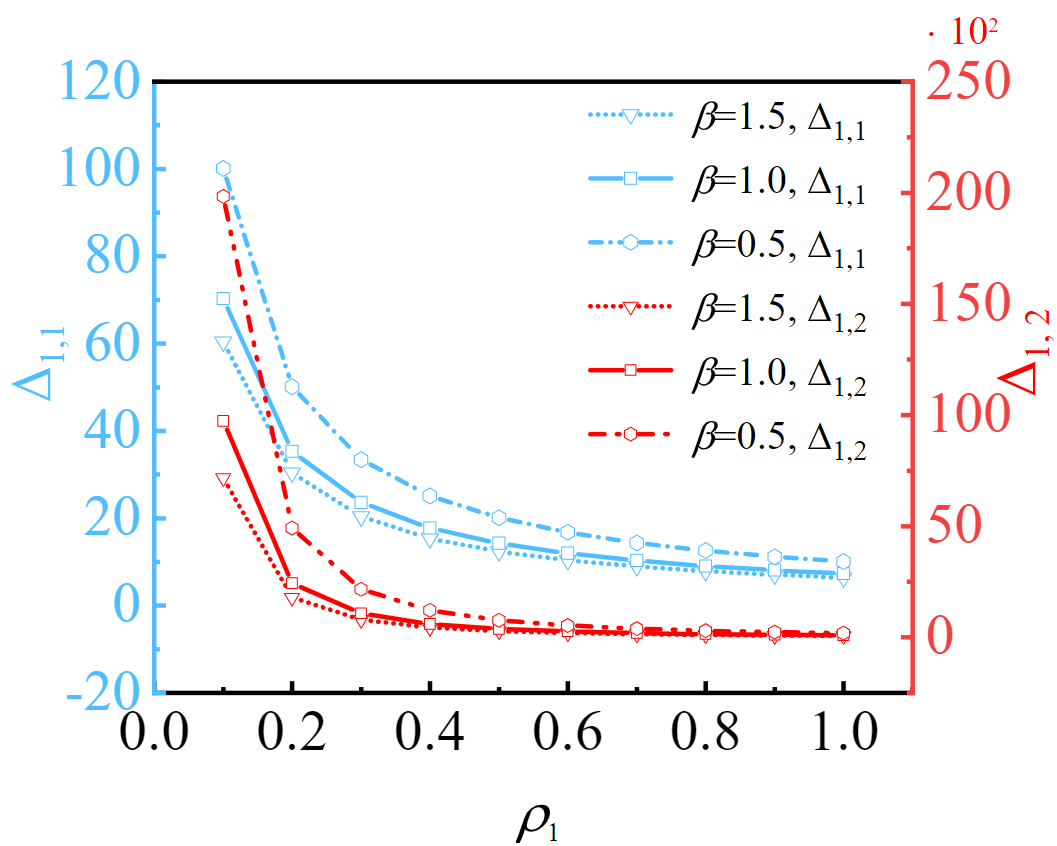
\includegraphics[width=0.48\textwidth]{1-2a}}
	\vspace{1pt}
	\subfigure[${\rho _1} + {\rho _2} = 4$]{\label{fig:subfig:1-2b}
		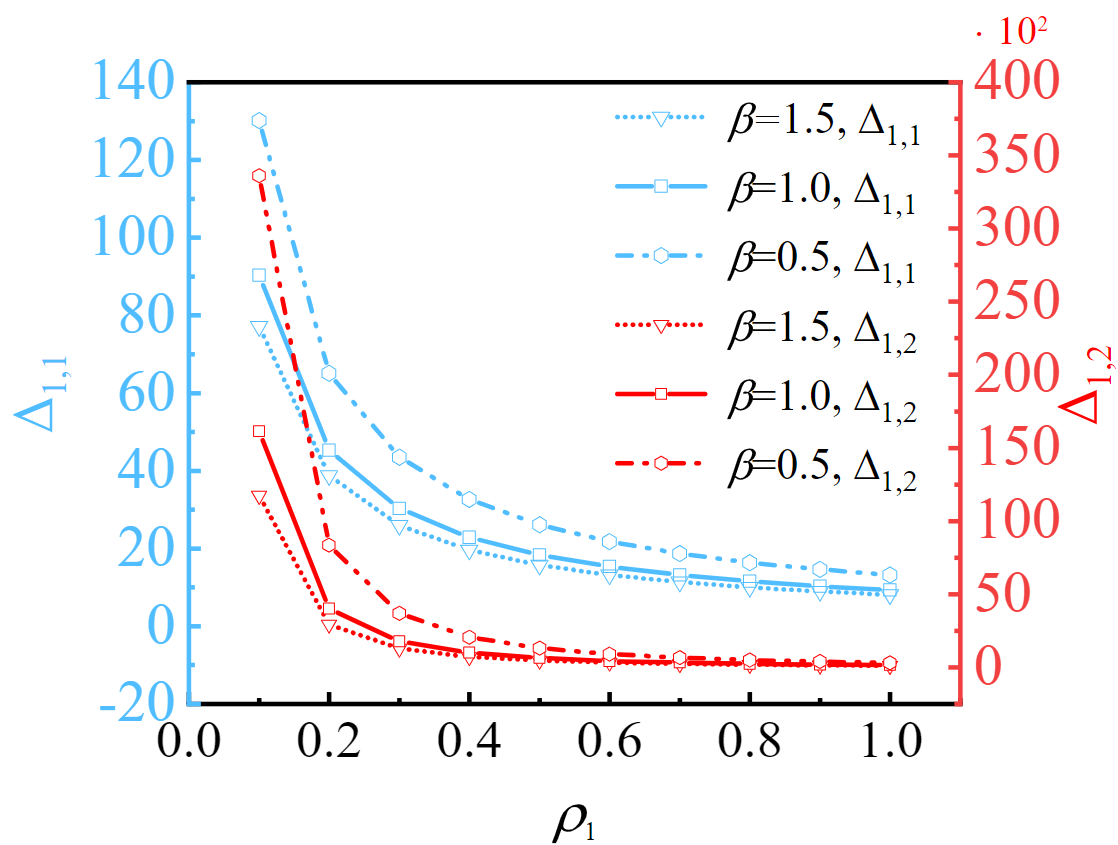
\includegraphics[width=0.48\textwidth]{1-2b}}
	\caption{$B = 1$,$\mu  = 1$设置下的平均 AoI${\Delta _{1,1}}$,方差 ${\Delta _{1,2}}$}\label{Fig1-2}
	\vspace*{10pt}
\end{figure}
图\ref{Fig1-2}给出$B = 1$设定下系统负载 $\rho$对 AoI 一阶矩,AoI 二阶矩的影响。分析图\ref{Fig1-2}可知,AoI 的一阶矩随 ${\rho_1}$的增大而逐渐降低。这时因为 ${\rho _1}$较小意味着系统中缺乏源${S_1}$新生成的状态更新包,这时服务器必须等待很长一段时间才能收到源${S_1}$的一个数据包,此时较长的等待时间会使得 AoI 的一阶矩较大。



\subsection{表的说明}

表\ref{Table1-1}显示了 5 个不同数据集的聚类准确率比较结果。该算法比较了在数据空间和用深度自动编码器编码后的特征空间的两种算法在数据的训练集和测试集上的聚类效果。从表中可以看出,不论任何数据集通过 SAE 编码后的聚类表现比直接进行聚类的表现更好,聚类准确率 ACC 有大幅度提高。这说明使用 SAE 提取数据的潜在特征,然后在数据集的特征空间进行聚类是有利的。这也说明了这些数据中存在着较多的冗余,经过了编码后的特征表现出更加清晰可分的结构。
\vspace{0.5em}
\begin{table}[ht!]
\centering
\caption { 不同聚类算法的聚类准确率比较 }\label{Table1-1}
\begin{tabular}{cccccc}
\hline \multirow{2}{*}{数据集 } & \multicolumn{2}{c}{SOM} & \multicolumn{2}{c}{提出的方法 } & \multirow{2}{*}{网络结构 } \\ \cline{2-5}
                 & 训练集        & 测试集        & 训练集         & 测试集  & \\
\hline  Iris     & 88.75 \% & 89.47 \% & 94.49 \% & 93.93 \% & \text { D-100-50-10-3 } \\
        Wine     & 91.52 \% & 90.59 \% & 96.24 \% & 95.56 \% & \text { D-100-50-10-3 } \\
        Isolet   & 58.82 \% & 57.68 \% & 66.42 \% & 64.7 \% & \text { D-500-100-30-26 } \\
        COIL-20  & 68.83 \% & 67.32 \% & 71.72 \% & 70.85 \% & \text { D-500-100-30-20 } \\
        MNIST    & 52.89 \% & 52.92 \% & 71.54 \% & 70.61 \% & \text { D-500-100-30-10 } \\
\hline
\end{tabular}
\end{table}

\textcolor[rgb]{1.00,0.00,0.00}{1. 表格一般应采用三线表(必要时可加辅助线),即表的上、下边线为单直线,线粗为 1.5 磅,第三条线为单直线,线粗为 1 磅。当三线表无法清晰表达时,可采用其他格式。}

\textcolor[rgb]{1.00,0.00,0.00}{2. 表中参数应标明量和单位的符号。表单元格中的文字一般用宋体 5 号或小 5 号字,居中(上下、左右均居中),单倍行距,段前空 3 磅,段后空 3 磅。不宜左右居中时,可采取两端对齐的方式。}

\textcolor[rgb]{1.00,0.00,0.00}{3. 表序与表名置于表的上方,用宋体 5 号字,居中,段前空 12 磅,段后空 6 磅,单倍行距,表序与表名文字之间空一个字符。如“表 3-1 XXX”,其中“表 3.1”是表序。}

\textcolor[rgb]{1.00,0.00,0.00}{4. 正文中表 1-1 前后没有空格。}

\textcolor[rgb]{1.00,0.00,0.00}{5. 表序、表名与表格应在同一页。当表格较大,不能在一页内打印时,可以“续表”形式另页打印,格式同前,只需在每页表序前加“续”字即可,例如“续表 3.1 XXX”。}

\textcolor[rgb]{1.00,0.00,0.00}{6. 表下方资料来源等文字说明,用宋体五号字,单倍行距,段前空 6 磅,段后空 12 磅。有续表时,资料来源注明在续表之下。}

\textcolor[rgb]{1.00,0.00,0.00}{7. 表格无特殊事由,一般不得截图。}

\subsection{公式的说明}

李雅普诺夫优化的本质是李雅普诺夫漂移,假设一个长度为$Ns$的系统队列,表示为向量组$Q\left( t \right) = \left( {{Q_1}\left( t \right),{Q_2}\left( t \right), \ldots ,{Q_{Ns}}\left( t \right)} \right)$。需要注意的是,这些队列包括实际队列和虚拟队列(它们与实际队列表现相同,但底层的物理含义与实际队列不同),此处所有队列变量都是非负的。为了度量$Q\left( t \right)$的总量,定义$Q\left( t \right)$的二次李雅普诺夫函数如下:
\begin{equation}\label{Eq1-1}
L\left( {Q\left( t \right)} \right) \buildrel \Delta \over = \frac{1}{2}\sum\limits_{n = 1}^{Ns} {{\theta _n}{Q_n}{{\left( t \right)}^2}},
\end{equation}
其中,${\theta _n},n = 1,2, \ldots ,Ns$是标记不同队列重要性的权重系数,${\theta _n}$必须为大于等于零的正值。通常当系统中所有队列的权重相同时,${\theta _n} = 1$。从上述可以得知,式\eqref{Eq1-1}中$L\left( {Q\left( t \right)} \right)$是非负的,当且仅当所有队列都为零时,它的值为零。

\textcolor[rgb]{1.00,0.00,0.00}{1. 表达式采用与正文相同的字号,单倍行距,居中或另起一段空两个汉字符书写(只能采用两种格式中的一种,全文须保持一致),段前空 6 磅,段后空 6 磅。}

\textcolor[rgb]{1.00,0.00,0.00}{2. 表达式的序号用括号,置于表达式右边行末,序号与表达式之间不加任何连线。}

\textcolor[rgb]{1.00,0.00,0.00}{3. 表达式在文字叙述中采用“式(3-1)”形式,在编号中用“(3-1)”形式。}

\textcolor[rgb]{1.00,0.00,0.00}{4. 公式中的字体为“Times New Roman”并斜体,大小可以在公式编辑器中自行设置,尽量让同一公式出现在同一行。}

\textcolor[rgb]{1.00,0.00,0.00}{5. 论文中出现的公式和参数字符一律用公式编辑器(如果没有用 mathtype)编写(不包括专有名词缩和其缩写),正文中公式出现显示不完整时,调整该行行间距为单倍行间距即可。}

\subsection{定理、推论、命题等的说明}

%定理
\begin{TheoremJXD}\label{Theorem1-1}
{考虑一个二次李雅普诺夫函数$L\left( {Q\left( t \right)} \right)$且$\mathbb{E}\left\{ {L\left( {Q\left( 0 \right)} \right)} \right\} < \infty $ ,假设此处的变量$B > 0$且$\varepsilon  \ge 0$,那么则有:
\begin{equation}\label{Eq1-2}
\Phi \left( {Q\left( t \right)} \right) \le B - \varepsilon \sum\limits_{n = 1}^{Ns} {\left| {{Q_n}\left( t \right)} \right|}.
\end{equation}
对所有的$Q\left( t \right)$都成立,从而有:
\begin{enumerate}
	\item {如果$\varepsilon  \ge 0$,则所有队列${Q_n}\left( t \right)$都是速率稳定的;}
	\item {如果$\varepsilon  > 0$,则所有队列都是强稳定的,并且有:
\begin{equation}\label{Eq1-3}
\mathop {\lim }\limits_{t \to \infty } \sup \frac{1}{t}\sum\limits_{\tau  = 0}^{t - 1} {\sum\limits_{n = 1}^{Ns}\mathbb{E} {\left\{ {\left| {{Q_n}\left( \tau  \right)} \right|} \right\}} }  \le \frac{B}{\varepsilon }.
\end{equation}	
}
\end{enumerate}
}
\end{TheoremJXD}
\vspace{0.5em}
上述\TheoremJXDref{Theorem1-1}给出了李雅普诺夫漂移界的队列稳定性条件。这个李雅普诺夫漂移的边界决定了系统中队列的稳定性。所有希望有效地保持稳定队列的算法都应该设计一种机制来实现这一界限。这一事实使得李雅普诺夫优化的框架易于识别。几乎所有利用李雅普诺夫优化的算法都可以分为两部分:第一部分努力满足上述定理的条件,从而使得队列稳定,而第二部分旨在实现一些系统目标,如吞吐量,功耗等,但这两部分并不是完全分开的,他们是由下面将要介绍的一些控制变量连接起来的。

%引理
\begin{LemmaJXD}\label{Lemma1-1}
考虑一个二次李雅普诺夫函数$L\left( {Q\left( t \right)} \right)$且$\mathbb{E}\left\{ {L\left( {Q\left( 0 \right)} \right)} \right\} < \infty $ ,假设此处的变量$B > 0$且$\varepsilon  \ge 0$,那么则有:
\begin{equation}\label{Eq1-4}
\Phi \left( {Q\left( t \right)} \right) \le B - \varepsilon \sum\limits_{n = 1}^{Ns} {\left| {{Q_n}\left( t \right)} \right|}.
\end{equation}
\end{LemmaJXD}
\vspace{0.5em}
上述\LemmaJXDref{Lemma1-1}给出了李雅普诺夫漂移界的队列稳定性条件。


%推论
\begin{CorollaryJXD}\label{Corollary1-1}
考虑一个二次李雅普诺夫函数$L\left( {Q\left( t \right)} \right)$且$\mathbb{E}\left\{ {L\left( {Q\left( 0 \right)} \right)} \right\} < \infty $ ,假设此处的变量$B > 0$且$\varepsilon  \ge 0$,那么则有:
\begin{equation}\label{Eq1-5}
\Phi \left( {Q\left( t \right)} \right) \le B - \varepsilon \sum\limits_{n = 1}^{Ns} {\left| {{Q_n}\left( t \right)} \right|}.
\end{equation}
\end{CorollaryJXD}
\vspace{0.5em}
上述\CorollaryJXDref{Corollary1-1}给出了李雅普诺夫漂移界的队列稳定性条件。


%定义
\begin{DefinitionJXD}\label{Definition1-1}
考虑一个二次李雅普诺夫函数$L\left( {Q\left( t \right)} \right)$且$\mathbb{E}\left\{ {L\left( {Q\left( 0 \right)} \right)} \right\} < \infty $ ,假设此处的变量$B > 0$且$\varepsilon  \ge 0$,那么则有:
\begin{equation}\label{Eq_2_3}
\Phi \left( {Q\left( t \right)} \right) \le B - \varepsilon \sum\limits_{n = 1}^{Ns} {\left| {{Q_n}\left( t \right)} \right|}.
\end{equation}
\end{DefinitionJXD}
\vspace{0.5em}
上述\DefinitionJXDref{Definition1-1}给出了李雅普诺夫漂移界的队列稳定性条件。


%命题
\begin{PropositionJXD}\label{Proposition1-1}
考虑一个二次李雅普诺夫函数$L\left( {Q\left( t \right)} \right)$且$\mathbb{E}\left\{ {L\left( {Q\left( 0 \right)} \right)} \right\} < \infty $ ,假设此处的变量$B > 0$且$\varepsilon  \ge 0$,那么则有:
\begin{equation}\label{Eq_2_3}
\Phi \left( {Q\left( t \right)} \right) \le B - \varepsilon \sum\limits_{n = 1}^{Ns} {\left| {{Q_n}\left( t \right)} \right|}.
\end{equation}
\end{PropositionJXD}
\vspace{0.5em}
上述\PropositionJXDref{Proposition1-1}给出了李雅普诺夫漂移界的队列稳定性条件。


\subsection{算法的描述}
在该算法中,提取特征阶段 SAE 采用逐层训练的方式对数据进行降维,在 mini-batch 模式下使用梯度下降进行优化,误差函数采用均方误差来减少损失。在训练过程中,SAE 首先通过第一层的编码器把原始数据编码特征,再通过解码函数把特征重构出输入数据,通过对原始数据和重构数据之间的误差进行比较,采用梯度下降对误差函数进行优化,更新本层编码器的参数,直到满足停止条件(误差足够小和到达最大迭代次数)后再依照第一层的训练过程进行下一层的训练任务。每层编码器都经过训练后训练完成。算法\ref{Algorithm1-1}详细描述了提取特征阶段的训练过程。在该算法中,提取特征阶段 SAE 采用逐层训练的方式对数据进行降维,在 mini-batch 模式下使用梯度下降进行优化,误差函数采用均方误差来减少损失。在训练过程中,SAE 首先通过第一层的编码器把原始数据编码特征,再通过解码函数把特征重构出输入数据,通过对原始数据和重构数据之间的误差进行比较,采用梯度下降对误差函数进行优化,更新本层编码器的参数,直到满足停止条件(误差足够小和到达最大迭代次数)后再依照第一层的训练过程进行下一层的训练任务。每层编码器都经过训练后训练完成。算法\ref{Algorithm1-1}详细描述了提取特征阶段的训练过程。
\vspace{10pt}
\begin{algorithm}[htb]	
	\setstretch{1.5}
 	\caption{训练堆叠自动编码器(提取特征阶段)}\label{Algorithm1-1}
	\begin{algorithmic}
		\wuhao
		\STATE \textbf{输入:}
        $\boldsymbol{X}=\left\{\boldsymbol{x}_1, \boldsymbol{x}_2, \cdots, \boldsymbol{x}_N\right\}$, batch 的大小 $b$, SAE 层数 $L$
        \STATE \textbf{输出:}	
         $\boldsymbol{H}=\left\{\boldsymbol{h}_1, \cdots, \boldsymbol{h}_N\right\}$ \\
        \vspace{0.3em}
        \hrule	
        \vspace{0.3em}		
        \STATE \textbf{1. }	
		初始化每层堆叠自动编码器的权值$\boldsymbol{W}_D^l$和偏差$\boldsymbol{b}_D^l$\\
        \STATE \textbf{2. }
        \textbf { for } $l \leftarrow 1$ \textbf { to } $L$ \textbf { do } \\
        \STATE \textbf{3. }
        \textbf { repeat} \\
        \STATE \textbf{4. }
        计算 $\boldsymbol{h}_i^{l-1}\left(\boldsymbol{h}_i^0=\boldsymbol{x}_i\right)$ 编码后的特征 $\boldsymbol{h}_i^l$ \\
        \STATE \textbf{5. }
        计算$\boldsymbol{h}_i^l$ 解码后产生的重构 $\tilde{\boldsymbol{h}}_i^{l-1}\left(\tilde{\boldsymbol{h}}_i^0=\tilde{\boldsymbol{x}}_i\right)$ \\
        \STATE \textbf{6. }
        计算$\boldsymbol{h}_i^l$和 $\tilde{\boldsymbol{h}}_i^{l-1}\left(\tilde{\boldsymbol{h}}_i^0=\tilde{\boldsymbol{x}}_i\right)$之间的误差  \\
        \STATE \textbf{7. }
        采用梯度下降优化更新参数$\theta^l=\left\{\boldsymbol{W}_D^l, \boldsymbol{b}_D^l\right\}$ \\
        \STATE \textbf{8. }
        \textbf {until} 满足停止条件 
        \STATE \textbf{9. }
        \textbf {end for}
	\end{algorithmic}
\end{algorithm}



\section{国内外研究现状}

参考文献的引用分为两种情况,一种是间接引用(上标)\cite{2004-David-Order},另一种是直接引用\mycite{2004-David-Order}。


主要包含以下几类参考文献:

1. 图书\mycite{2004-David-Order}

2. 期刊论文\mycite{2022-Jiao-TVT,2022-Guo-SP}

3. 会议论文\mycite{2015-Pappas-ICC}

4. 学位论文\mycite{2018-BUT}

其余请大家根据需要自行补充


\section{本文研究内容}

本文主要的研究内容如下:

(1)……

(2)

(3)


\section{论文结构安排}

本文从室内位置服务研究背景和无线定位算法研究现状出发,重点针对基于 Wi-Fi 的室内定位算法开展了深入的学习研究。论文结构安排如下:

第 1 章 绪论。首先介绍了基于位置服务中室内定位技术的研究背景和意义,然后简要概述了基于位置服务的体系结构、定位算法研究现状,最后阐述了本论文主要工作和结构安排。




